\documentclass[aip,jcp,reprint,twocolumn]{revtex4-1}
\usepackage{amssymb}
\usepackage{amsmath}
\usepackage{amsfonts}
\usepackage{graphicx}
\usepackage{tikz}
\usepackage{mhchem}


\usepackage[size=small]{caption}
%\usepackage{etoolbox}
%\AtBeginEnvironment{algorithm}{\noindent\hrulefill\par\nobreak\vskip-5pt}

\usepackage{newfloat}
\DeclareFloatingEnvironment[
    fileext=loa,
    listname=List of Algorithms,
    name=ALGORITHM,
    placement=tbhp,
]{algorithm}

\DeclareCaptionFormat{algorithms}{\vskip-15pt\hrulefill\par#1#2#3\vskip-6pt\hrulefill}
\captionsetup[algorithm]{singlelinecheck=off,format=algorithms}

%\usepackage{float}
%\floatstyle{ruled}
%\newfloat{algorithm}{t}{loa}
%\floatname{algorithm}{Algorithm}

\begin{document}

\title{Intrinsic Variables and State Reconstruction in Multiscale Simulations}

%\author{}
%\email{}
%\affiliation{}

\date{\today}

\begin{abstract}
Finding informative low-dimensional descriptions of high dimensional simulation data
(like the ones arising in molecular dynamics or kinetic Monte Carlo simulations of
physical/chemical processes) is crucial in understanding physical phenomena, and can
also dramatically assist in accelerating the simulations themselves.
%
In this paper, we discuss and illustrate the use of nonlinear intrinsic variables (NIVs)
in the mining of high-dimensional multiscale simulation data.
%
In particular, we focus on the way that NIVs allow us to functionally merge different
simulation ensembles, and {\em different partial observations of these ensembles}, as well
as to infer variables not explicitly measured.
%
The approach relies on certain simple features of the underlying process variability to
filter out measurement noise and systematically recover a unique reference coordinate frame.
%
We illustrate the approach through two distinct sets of multiscale atomistic simulations: a fast/slow
time scale simulation of an enzyme reaction network, and a molecular
dynamics simulation of alanine dipeptide in explicit water.

\end{abstract}

\keywords{Intrinsic variables, partial observations, complex dynamical systems}

\maketitle

\section{Introduction}
The last decade has witnessed extensive advances in dimensionality reduction techniques:
finding meaningful low-dimensional descriptions of high-dimensional data.
%
These developments have the potential to significantly enable the computational exploration
of phyiscochemical problems.
%
If the (high-dimensional) data $Y(t)$ arise from, say, a
molecular dynamics simulation of a macromolecule in solution, or from the stochastic
simulation of a complex chemical reaction scheme, the detection of a few good, coarse-grained
``reduction coordinates" $x(t)$ is invaluable in understanding and predicting system behavior.

%
While the benefits from such reduced descriptions are manifest, a crucial shortcoming of
such data-driven reduction coordinates is their dependence on the specific data set processed,
and not only on the physical model in question.
%
It is well known that, even in the simple linear case of Principal Component Analysis,
different data sets on the same low-dimensional hyperplane in the ambient space $Y$
will lead to different basis vectors - in effect, to different $x$.
%
While this can be easily fixed by a linear transformation, the problem becomes
exacerbated when the low-dimensional space is curved (a manifold, rather than a hyperplane)
and when different data ensembles are obtained using different instrumental modalities
(say, when one wants to merge molecular dynamics data with spectral information).
%
Clearly, the ability to systematically construct a {\em unique, consistent} reduction
coordinate set, shared by all measurement ensembles and observation modalities -
what we call a (Nonlinear) Intrinsic Variable Set - is invaluable.
%
Embedding data in such a coordinate system allows us to naturally merge different observations of the same system;
more importantly, it enables the construction of an empirical mapping between these different
observation ensembles, allowing us to complete partial measurements through the construction
of nonlinear observers of unmeasured variables.
%
This latter empirical mapping requires good interpolation tools in embedding space; to this
end we will demonstrate here the use of a multiscale Laplacian Pyramid approach \cite{rabin2012heterogeneous}.
%
We chose two distinct multiscale illustrative examples. The first is a simulation
of two Goldbeter-Koshland modules in an enzyme kinetics model \cite{zagaris2012stability} using Gillespie's Stochastic Simulation
Algorithm (SSA); in certain parameter regimes, separation of time scales is known
to reduce this model to an effective two-dimensional description.
%
Although this example is rather simple, it will serve as a nice introduction to our techniques and highlight the main features of the algorithms.
%
The second example is a molecular dynamics
simulation (in explicit water) of a simple peptide fragment (alanine dipeptide) whose folding
dynamics are known to be described through a small set of physical observables.
%
This example will demonstrate how our techniques outperform more common techniques, such as diffusion maps for dimensionality reduction
and nearest neighbor interpolation for reconstruction.
%
The paper is structured as follows: in Section \ref{sec:NIV} we present the Nonlinear Intrinsic Variable formulation and
the associated inference method. 
%
Section \ref{sec:LapPyr} contains our discussion of Laplacian Pyramids that
will be used for the completion of partial observations. 
%
Section \ref{sec:examples} contain the results
of applying the approach to simulation data from our two illustrative examples. 
%
We conclude with
a summary and discussion of open issues in Section \ref{sec:conclusions}.

\section{Nonlinear Intrinsic Variables} \label{sec:NIV}

\subsection{Overview}
Let $\mathbf{Y}(t)$ be a high-dimensional measured process in $\mathbb{R}^n$ consisting of $n$ observable variables.
The measured process is assumed to be a manifestation in an observable domain of a low-dimensional diffusion process. Thus, it can be expressed by
\begin{equation}
	\mathbf{Y}(t) = f(\mathbf{x}(t))
\end{equation}
where $f:\mathbb{R}^d \rightarrow \mathbb{R}^n$ is an unknown (possibly nonlinear) function and $\mathbf{x}(t)$ is a diffusion process that consists of $d$ underlying variables.
%
The dynamics of the diffusion process in each of its underlying variables are described by normalized stochastic differential equations as
\begin{equation}
	d x_i(t) = a_i (x_i(t)) dt + d w_i(t), \ i=1,\ldots,d
\end{equation}
where $a_i$ are unknown drift functions and $\dot{w}_i(t)$ are independent white noises TODO: should there be a dot here?.

Given a sequence of samples $\mathbf{Y}(t), \ t=1,\ldots,T$, we present an empirical method to construct a unique and consistent reduction coordinate set, represented here by $\mathbf{x}(t)$. 
%
By relying on the fact that the empirical method we will describe is independent of the observation function $f$, we present the notion of intrinsic modeling and refer to the coordinates of $\mathbf{x}(t)$ as a Nonlinear Intrinsic Variable (NIV) set.
%
The available samples $\mathbf{Y}(t)$ may be the product of different measurement functions $f$ in various observable domains, or they maybe partial measurements consisting of merely a subset of the coordinates of the observable domains.
%
The idea would be to empirically construct a NIV coordinate system driven entirely by measurements that is invariant to the observation modality (see Figure \ref{fig:IntrinsicIllustration} for illustration).

The presented method consists of the following main principles. 
%
(1) The underlying diffusion process implies that a short trajectory of successive samples mainly consists of diffusion noise, and hence, creates a ``sphere" of samples in the underlying domain. 
%
This sphere is mapped to an ellipse in the observable domain by the measurement function $f$. 
%
In this work, the identification of the associated ellipse of samples according to the time labels enables to explore and learn the tangent planes of the observable manifolds via the principal components of the covariance matrices of the samples in these ellipses. 
%
(2) The principal directions of the tangent planes are utilized to define a Riemannian metric that is shown to be locally invariant to the measurement function $f$. 
%
(3) The NIV are constructed through the eigenvalue decomposition of a Laplace operator that is built upon a pairwise affinity between the samples, defined using the Riemannian metric.

\begin{figure*}[ht]
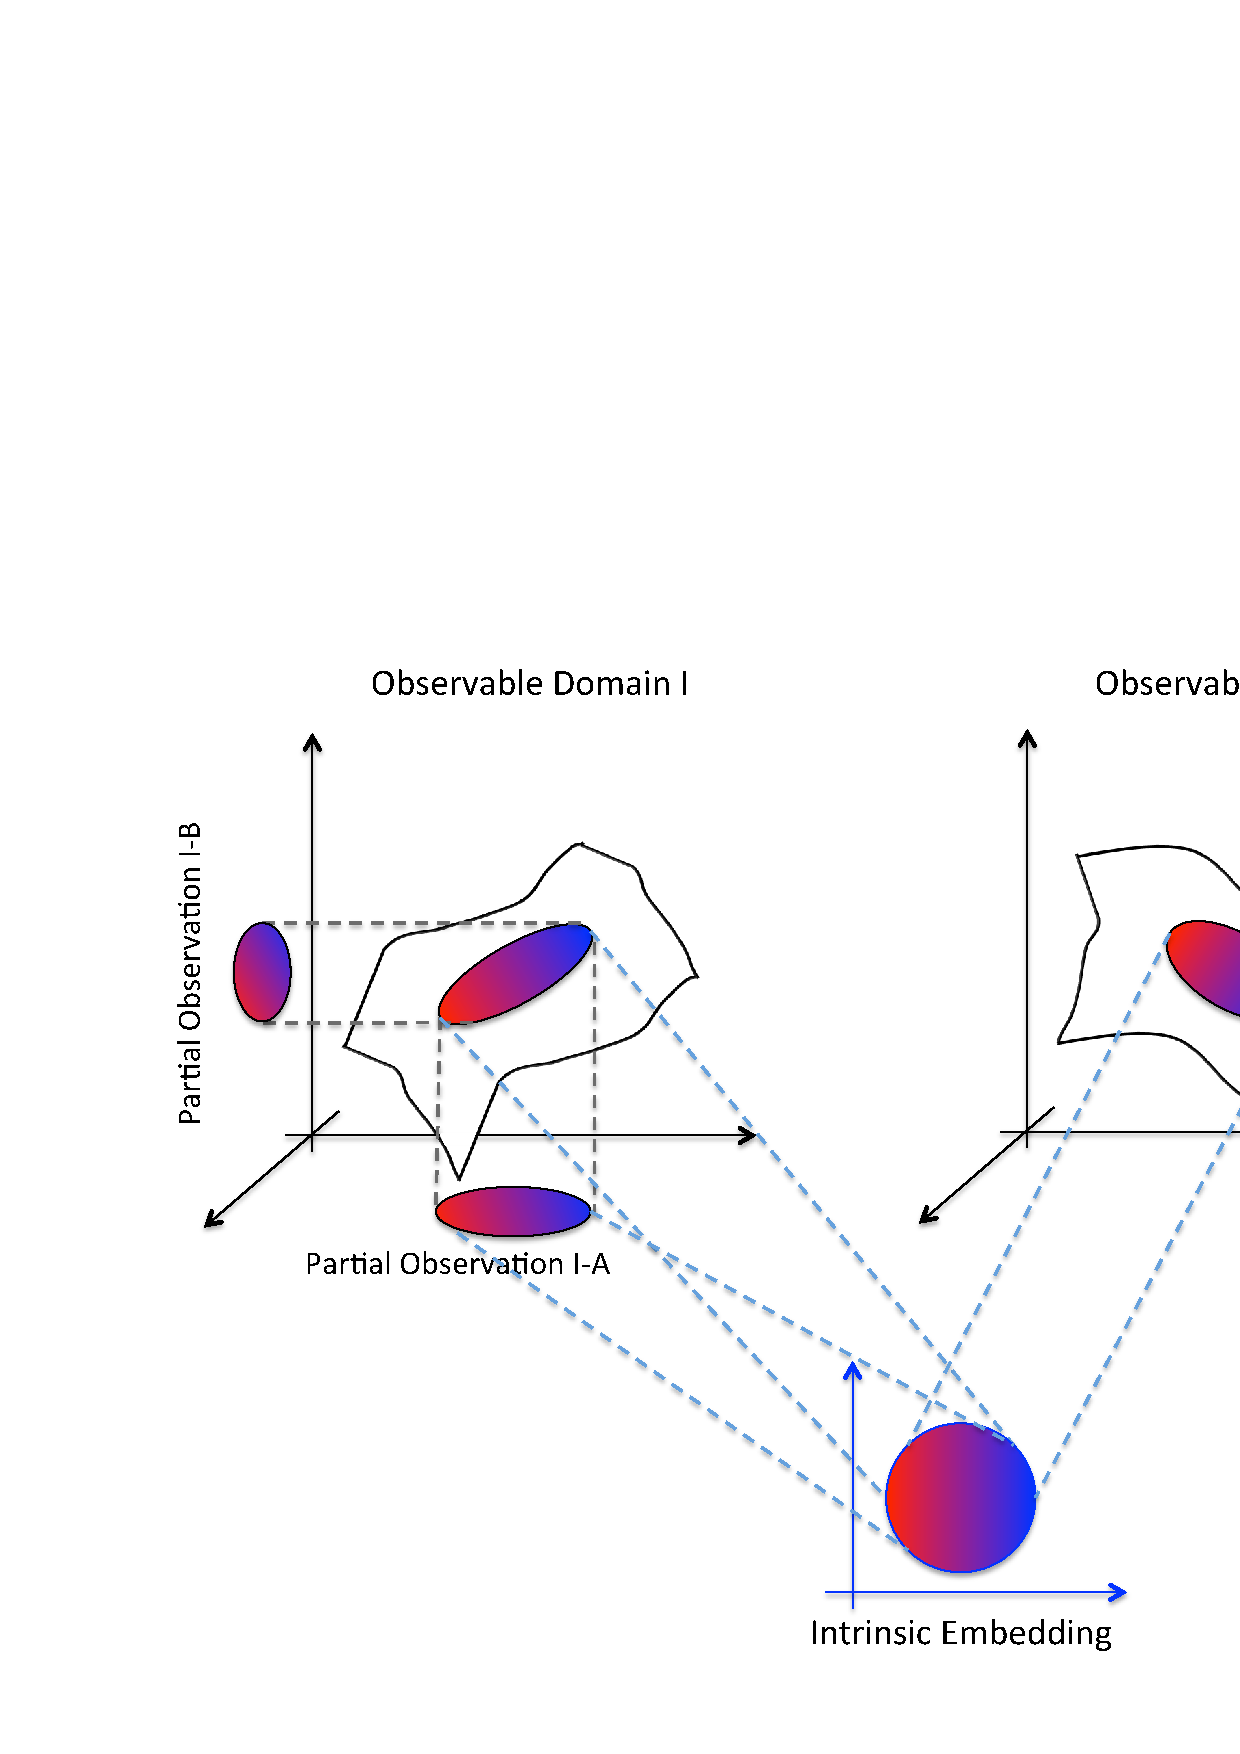
\includegraphics[width=0.7\textwidth]{IntrinsicEmbeddingIllustration2}
\caption{Illustration of the nonlinear embedding that yields an intrinsic representation independent of the measurement modality. (Bottom) The underlying variables in which the diffusion parameters are independent with unit variance. The circle illustrates successive sample in a short burst/trajectory in time that create a sphere on the parametric manifold. (Top Left) The first set of observed variables. The ellipse illustrates the mapping of the sphere of the underlying samples into the observable domain via the first observation modality. In this domain, we illustrate that the observations might be partial, i.e., consist of merely a subset of the observed domain variables. (Top Right) The second set of observable variables. The ellipse illustrates the mapping of the sphere of the underlying samples into a different observable domain via a second observation modality.}
\label{fig:IntrinsicIllustration}
\end{figure*}

\subsection{Mahalanobis Distance}
\label{subsec:mahalanobis}

Let $\mathbf{C}(t)$ be the covariance matrix associated with the measured sample $\mathbf{Y}(t)$. In practice, the covariance matrix can be estimated from a short trajectory of samples in time around the sample $\mathbf{Y}(t)$ by
\begin{equation}
	\widehat{\mathbf{C}}(t) = \sum \limits _{\tau = t-L}^{t+L} (\mathbf{Y}(\tau) - \widehat{\boldsymbol{\mu}}(t))(\mathbf{Y}(\tau) - \widehat{\boldsymbol{\mu}}(t))^T
	\label{eq:cov}
\end{equation}
where $\widehat{\boldsymbol{\mu}}(t)$ is the empirical mean of the samples.

In particular, we define a Riemannian metric between a pair of samples using the associated covariance matrices as
\begin{align}
	d(\mathbf{Y}(t), \mathbf{Y}(\tau)) &= 2 (\mathbf{Y}(t) - \mathbf{Y}(\tau))^T(\mathbf{C}(t) + \mathbf{C}(\tau))^{-1} \nonumber \\
	&\times (\mathbf{Y}(t) - \mathbf{Y}(\tau)).
	\label{eq:mahalanobis}
\end{align}
This metric \eqref{eq:mahalanobis} is called the Mahalanobis distance.
%
As previously described, the covariance matrices convey the local variability of the measurements and are utilized to explore and learn the tangent planes of the observable manifold.
%
This information is then utilized in \eqref{eq:mahalanobis} to compare a pair of points according to the directions of their respected tangent planes.

The Mahalanobis distance is invariant under linear transformations.
%
Thus, by assuming that the observation function $f$ is bi-Lipschitz and smooth and by using local linearization of the function, i.e., $\mathbf{Y}(t) = \mathbf{J}(t) \mathbf{x}(t) + \boldsymbol{\epsilon}(t)$ where $\mathbf{J}(t)$ is the Jacobian of $f(\mathbf{x}(t))$ and $\boldsymbol{\epsilon}(t)$ is the residual consisting of higher-order terms, it was shown by Singer and Coifman \cite{singer2008non} that $\mathbf{C}(t) = \mathbf{J}(t)\mathbf{J}^T(t)$ and that the Mahalanobis distance approximates the Euclidean distance between the corresponding samples of the underlying process to a second order, i.e.,
\begin{equation}
	\| \mathbf{x}(t) - \mathbf{x}(\tau) \|^2 = d^2(\mathbf{Y}(t), \mathbf{Y}(\tau)) + \mathcal{O}(\| \mathbf{Y}(t) - \mathbf{Y}(\tau)\|^4).
\end{equation}
%
This result implies that the Mahalanobis distance is invariant to the measurement function $f$, and hence, 
it yields the same distances between samples obtained under different observation modalities or even partial observations.

\subsection{Laplace Operator}
The Mahalanobis distance described in Section \ref{subsec:mahalanobis} enables to compare the observations in terms of the intrinsic variables of the associated underlying diffusion process.
%
In this section, we recover the underlying process itself from the pairwise Euclidean distances through the eigenvectors of a Laplace operator.

Let $\mathbf{W}$ be a pairwise affinity matrix (kernel) based on a Gaussian, whose $(t,\tau)$-th element is given by
\begin{equation}
	W_{t,\tau} = \exp \left\{ - \frac{ d^2(\mathbf{Y}(t), \mathbf{Y}(\tau) )} {\varepsilon}\right\}
	\label{eq:kernel}
\end{equation}
where $\varepsilon$ is the kernel scale, which can be set according to \cite{coifman2008graph}.
%
Let $\mathbf{D}$ be a diagonal matrix whose diagonal elements are the sums of rows of $\mathbf{W}$, and let $\mathbf{W}^{\mathrm{norm}} = \mathbf{D}^{-1/2}\mathbf{W}\mathbf{D}^{-1/2}$ be a normalized kernel that shares its eigenvectors with the normalize graph-Laplacian $\mathbf{I}-\mathbf{W}^{\mathrm{norm}}$ \cite{chung1997spectral}. 
%
These eigenvectors $\psi_j$ reveal the underlying structure of the data TODO:cite. 
%
Specifically, the $i$-th coordinate of the $j$-th eigenvector can be associated with an intrinsic coordinate $j$ of the sample $\mathbf{x}(i)$ of the underlying process. 
%
The above steps to construct the nonlinear intrinsic variables are summarized in Algorithm \ref{algo}.

%TODO: do we need to describe the extension procedure?! - the recovery of the intrinsic variables through the eigenvalue decomposition (EVD) of the Laplace operator is computationally heavy...\\
TODO: we can discuss the probabilistic interpretation and explicitly state that we set the kernel scale to the median of the kernel.\\

Each eigenvector then describes an intrinsic variable for the data set of interest.
%
Because eigenvectors can be determined up to a scaling factor, we must scale the eigenvectors from different data sets in a way so that the resulting embeddings are consistent.
%
We first scale the eigenvectors so that the norm of the each eigenvector is equal to the cardinality of the data set.
%
Intuitively, a data set that has twice as many samples as another data set, but the same underlying density and shape, should have twice the norm.
%
Still, the embedding eigenevctors for two identical data sets could differ by a sign.
%
Reconciling the signs for the embeddings of different data sets can be done in several ways and is somewhat problem-specific.
%
For example, if the mean of the embedding is sufficiently far from 0, the signs can be chosen such that the mean of each eigenvector is greater than 0;
alternatively, we can construct the data sets such that a few points are common between both data sets, and the sign of each eigenvector can be chosen to optimize the consistency of the embeddings of these common points.

\begin{algorithm}[th!]
\caption{Nonlinear Intrinsic Variables Construction}
\begin{enumerate}

\item
Obtain a sequence of high-dimensional observation samples $\mathbf{Y}(t)$.

\item
Compute the empirical covariance matrix $\widehat{\mathbf{C}}(t)$ of each sample $\mathbf{Y}(t)$ in a short windows in time according to \eqref{eq:cov}.

\item
Using the samples and their associated covariance matrices, compute the Mahalanobis distance between the observations \eqref{eq:mahalanobis} .

\item
Build the pairwise affinity matrix $\mathbf{W}$ and the corresponding normalized kernel $\mathbf{W}^{(\mathrm{norm})}$ (\ref{eq:kernel}).

\item
Apply EVD on the normalized kernel and view the values of its principal eigenvector as the intrinsic variables of the given observations.

\end{enumerate}
\hrule
\label{algo}
\end{algorithm}

\section{Laplacian Pyramids} \label{sec:LapPyr}

Laplacian Pyramids (LP) is a multi-scale algorithm for approximating and extending an empirical function $f$ defined on a set of points.
%
The algorithm uses Laplacian kernels of decreasing widths to create multi-scale representations of $f$.
%
These representations can be easily extended to new data points.
%
This type of multi-scale representation was introduced by Burt and Adelson \cite{burt1983laplacian} for image coding,
and was later shown to be a tight frame by Do and Veterli \cite{do2003framing}.
%
Recently, LP was used to extend nonlinear embedding coordinates to new high-dimensional data points \cite{rabin2012heterogeneous}.
%
We will first review the LP algorithm for approximating and extending a one-dimensional function.
%
We will then describe the application of LP in the context of this work - extending a high-dimensional function that is known on a set of points which lie in a low-dimensional space.

Let $f: \Gamma \rightarrow \mathbb{R}^d$ be a function that is known on a subset of points $S \subset \Gamma$.
%
A coarse representation of $f$ is generated using a coarse smoothing operator $P_0$.
%
The smoothing operator $P_0$ is a normalized, coarse Laplacian kernel, defined by $p_0(t,\tau)= s_0^{-1}(t)w_0(t,\tau)$, where $w_0(t,\tau)=e^{-d^2(t,\tau) / \sigma_0}$. 
%
The pairwise distance $d(t,\tau)$ is typically the Euclidian distance. 
%
The parameter $\sigma_0$ is set to be large compared to the values of $d(t,\tau)$  and $s_0^{-1}(t)=\sum_{\tau \in S}w_0(t,\tau)$ is the normalizing term. 
%
The application of $P_0$ to $f$ yields a coarse representation of the function, which we denote by $f_0=P_0(f)$.

The difference $\delta_1 = f-P_0(f)$ is input for the next iteration of the algorithm, 
which uses the smoothing operator $P_1$, $P_1 \propto e^{-d^2(t,\tau)^2 / 2^{-1} \sigma_0}$, to construct a coarse representation of $\delta_1$.
%
The obtained  representation of $\delta_1$, $P_1(\delta_1)$ together with the result of the previous iteration $f_0 = P_0(f)$ 
yields a new, finer representation of $f$, $f_1 = P_0(f) + P_1(\delta_1)$.

In an iterative manner, multi-scales representations of the function $f$, denoted by $f_l$ are constructed (see Eq. \eqref{eq:LP_multi_scale}). 
%
As $l$ grows, the approximation is of a finer resolution because $P_l \propto e^{-d^2(t,\tau) / 2^{-l} \sigma_0}$ uses a Laplacian kernel of a finer width. 
%
The iterations stop when the difference between $f$ and $f_l$ is smaller than a pre-defined error threshold.

\begin{equation} \label{eq:LP_multi_scale}
 \begin{array}{cl}
\mbox{scale 0:} & f_0 = P_0(f) \\
\mbox{scale 1:} & f_1 = P_0(f) + P_1(\delta_1) \\
: & : \\
\mbox{scale l:} & f_l = P_0(f) + \sum_{k=1}^{l}P_k(\delta_k)\\
\end{array}
\end{equation}

The representations $f_0$, $f_1$,..$f_l$ can be extended to a new point $\tilde{t} \in \Gamma \backslash S $ by extending the operators $P_0, P_1,\ldots,P_l$. 
%
For example, $f_0(\tilde{t}) = \sum_{t \in S} p_0(\tilde{t}, t)f(t)$ and
$f_1(\tilde{t}) = f_0(\tilde{t}) + \sum_{(t \in S)}p_1(\tilde{t}, t)\delta_1(t)$.

\begin{widetext}
Figure \ref{fig:LP_ex} displays an illustrative example of the algorithm, when applied to the function 
 \begin{equation} \label{eq:LP_example}
f(x) = \left\{
\begin{array}{l l}
-0.02(x-4\pi)^2 + \sin(x) &  0 \le x \le 4\pi \\
-0.02(x-4\pi)^2 + \sin(x) + 0.5 \sin(3x) &  4\pi < x \le 7.5 \pi \\
-0.02(x-4\pi)^2 + \sin(x) + 0.5 \sin(3x) +0.25 \sin(9x) &  7.5 \pi < x \le 10 \pi
\end{array}
\right.
\end{equation}
that contains several scales. 
%
The coarse regions of the function ( $0 \le x \le 4\pi$ ) are well approximated by a small number of scales. 
%
As the function becomes more oscillatory ( $\pi \le x \le 7.5\pi$ and $7.5\pi \le x \le 10\pi$), 
a finer representation, (meaning a larger number of scales  $l$ )  is required to capture its behavior.
\end{widetext}

In this work, LP is applied to extend a high-dimensional function $f:\mathbb{R}^d \rightarrow \mathbb{R}^n$, which maps a set of points in the NIV space to their values $\mathbf{Y}(t)$ in the observable space.
%
Let $\Psi(t) = \left(\psi_1(t),\psi_2(t),\ldots,\psi_d(t)\right)$ be the set of NIV's that were constructed from the data samples $\mathbf{Y}(t)$, as described in Algorithm \ref{algo}. 
%
The values of function $f:\mathbb{R}^d \rightarrow \mathbb{R}^n$ are known on the subset $S = \{\Psi(t)\}$, with $f(\Psi(t)) = Y(t)$.

A na\"{\i}ve way to extend $f$ to a new data point $\Psi(\tilde{t})$ is find the point's nearest neighbors in NIV space and average their function values. 
%
A different, point-wise adaptive approach is described by Buchman {\em et al} \cite{buchman2011high}; 
high-dimensional hurricane tracks were estimated from low dimensional embedding coordinates using a weighted average of the points close to $\Psi(\tilde{t})$ in the embedded space. 
%
However, this point-wise adaptation requires setting the nearest neighborhood radius parameter for every point.

The LP algorithm automatically finds the nearest neighborhood radius for each new point $\Psi(\tilde{t})$. 
%
This radius will be large in smooth regions of the function, and small in regions in which $f$ contains higher frequency components. 
%
The LP approximation of a new, high dimensional value $Y(\tilde{t})$, is calculated by a weighted average of the function values that belong to the neighboring points. 
%
The weights are based on the pairwise distances in the intrinsic, low-dimensional space. 
%
In practice, a set of smoothing operators $P_0, P_1, \ldots, P_l$
\begin{equation} \label{eq:LP_multi_scale_app}
P_l \propto e^{-d(\Psi(t),\Psi(\tau))^2 / \sigma_0 \cdot 2^{-l}}
\end{equation}
are constructed and later extended to create the multiscale approximations as defined in Eq. \ref{eq:LP_multi_scale}.
%
The LP algorithm for inverse mapping is summarized in Algorithm \ref{algo_LP}.

\begin{algorithm}[th!]
\caption{Laplacian Pyramids for Inverse Mapping}
\begin{enumerate}

\item
Construct a set of smoothing operators $P_0, P_1, \ldots, P_l$  based on intrinsic pairwise distances $d(\Psi(t),\Psi(\tau))$.


\item
Use the smoothing operators to obtain a multiscale representation (see Eq. \ref{eq:LP_multi_scale_app}) of $f:\Psi(t) \rightarrow Y(t)$.

\item Given a new point $\Psi(\tilde{t})$ in NIV, extend the smoothing operators $P_0, P_1, \ldots, P_l$  by
$p_l(\Psi(\tilde{t}), \Psi(t)) = s_0^{-1}(\Psi(t))w_0(\Psi(\tilde{t}),\Psi(t))$.

\item
Use the extended smoothing operators to approximate the value of $f_l(\tilde{t}) = f_0(\tilde{t}) + \sum_{k}\sum_{(t \in S)}p_k(\tilde{t}, t)\delta_k(t)$


\item
The value $Y(\tilde{t})$ is approximated by $f_l(\Psi(\tilde{t}))$.

\end{enumerate}
\hrule
\label{algo_LP}
\end{algorithm}


\begin{figure*}[ht]
\includegraphics[width=0.2\textwidth]{LP_figures/Scale3_S2}
\includegraphics[width=0.2\textwidth]{LP_figures/Scale5_S2}
\includegraphics[width=0.2\textwidth]{LP_figures/Scale8_S2}
\includegraphics[width=0.2\textwidth]{LP_figures/Scale11_S2}
\caption{Approximation of function $f(x)$ as defined in \eqref{eq:LP_example} for scales 3, 5, 8, and 11 using Laplacian Pyramids (top, the true function is shown in blue and the Laplacian Pyramids approximation in shown in black), and the residual error in the approximation (bottom, shown in red).}
\label{fig:LP_ex}
\end{figure*}

\section{Models and Results} \label{sec:examples}

\subsection{Chemical Reaction Network}

We first consider a chemical reaction network of multiple enzyme-substrate interactions \cite{zagaris2012stability}.
%
The equations that govern the network are\\
\begin{center}
\ce{$E$ + $S$ <=>[e_1][e_{-1}] $E:S$ ->[e_2][] $E$ + $S^{*}$}\\
\ce{$S$ + $E$ <=>[b_1][b_{-1}] $S:E$ ->[b_2][] $S$ + $E^{*}$}\\
\ce{$D$ + $S^{*}$ <=>[d_1][d_{-1}] $D:S^{*}$ ->[d_2][] $D$ + $S$}\\
\ce{$F$ + $E^{*}$ <=>[f_1][f_{-1}] $F:E^{*}$ ->[f_2][] $F$ + $E$}\\
\end{center}

The $^{*}$ denote activated forms of the various species, and the : denote complexes formed between two species; the complexes $E:S$ and $S:E$ are not equivalent.

There are 10 species in this reaction system;
however, one can write four conservation equations (since total $E$, $S$, $D$, and $F$ are all conserved) to reduce the system to 6 dimensions.
%
%We assume each reaction follows an elementary rate law.
%
%We use the parameters $b_1=5$, $d_1=0.0009$, $e_1=0.1$, $f_1=0.1$, $b_{-1} = 10.6$, $d_{-1}=0.05$, $e_{-1}=0.5$, $f_{-1} =0.01$, $b_2=0.4$, $d_2=0.85$, $e_2=0.05$, and $f_2=2$.
%
%We take $S_T=E_T=D_T=1$, and $F_T=0.02$, where $S_T$, $E_T$, $D_T$, and $F_T$ are total concentrations of $S$, $E$, $D$, and $F$, respectively.
%
In the parameter regime we consider, the system exhibits a separation of timescales, so that initial conditions quickly approach a two-dimensional manifold;
details about the specific parameters can be found in Appendix \ref{app:rxn}.
%
%The relevant timescales around the steady state ($-1/\lambda_i$, where $\lambda_i$ are the eigenvalues of the Hessian) are 1176, 9.731, 1.594, 1.111, 0.4975, 0.06498.

Although the dynamics of chemical reaction networks are typically described by a system of ODEs, the ODEs are only an approximation that holds in the limit of a large number of molecules.
%
When the number of molecules is small, the system is inherently stochastic and its dynamics can be simulated using the Gillespie's Stochastic Simulation Algorithm (SSA) \cite{gillespie1977exact}.
%
We can control the level of noise by adjusting the volume $V$, and therefore adjusting the number of molecules, in the system (in our simulations, we take $V=10^5$).
%
We take the volume small enough so that we can still see appreciable stochasticity in small simulation bursts, but large enough so that the underlying two-dimensional manifold is (relatively) smooth.

We generate 3000 random initial conditions $\mathbf{Y}^{full}_0(1), \dots, \mathbf{Y}^{full}_0(3000) \in \mathbb{R}^6$, enforcing that all concentrations must be non-negative
(we take the order of the components in the vector $\mathbf{Y}^{full}_0(t)$ to be $S$, $E$, $E:S$, $S:E$, $D:S^{*}$, $F:E^{*}$).
%
We integrate each point $\mathbf{Y}^{full}_0(t)$ forward for 10 time units using the SSA to obtain point the $\mathbf{Y}^{full}(t) \in \mathbb{R}^6$;
10 time units is sufficiently long for the initial points to converge to the two-dimensional manifold,
but not long enough for the points to converge to a one-dimensional curve or to the final steady state.
%
We take $\mathbf{Y}^{full}(1), \dots, \mathbf{Y}^{full}(3000)$ to be representative points on the underlying two-dimensional manifold;
three-dimensional projections of the resulting manifold are shown in Figure \ref{fig:rxn_manifolds}.
%
From each manifold point $\mathbf{Y}^{full}(t)$, we run 20 short simulations, each for 0.2 time units.
%
We denote the endpoints from the short simulations as $\widetilde{\mathbf{Y}}^{full}(t, 1), \dots, \widetilde{\mathbf{Y}}^{full}(t, 20)$.

\begin{figure*}[ht]
  \includegraphics[height=6cm]{rxn_figures/rxn_manifold1}\llap{\raisebox{3.5cm}{\includegraphics[height=2.5cm]{rxn_figures/rxn_manifold1_2}}}
  \includegraphics[height=6cm]{rxn_figures/rxn_manifold2}\llap{\raisebox{3.5cm}{\includegraphics[height=2.5cm]{rxn_figures/rxn_manifold2_2}}} \\
  \includegraphics[height=6cm]{rxn_figures/rxn_manifold3}\llap{\raisebox{3.5cm}{\includegraphics[height=2.5cm]{rxn_figures/rxn_manifold3_2}}}
  \includegraphics[height=6cm]{rxn_figures/rxn_manifold4}\llap{\raisebox{3.5cm}{\includegraphics[height=2.5cm]{rxn_figures/rxn_manifold4_2}}} \\
    \caption{Projections of the manifold from stochastic simulation of the chemical reaction network. The insets show rotations of the projections to illustrate the two-dimensionality of the manifold.}
    \label{fig:rxn_manifolds}
\end{figure*}

We consider two different data sets from our simulations.
%
Data set 1, denoted $\mathbf{Y}_1(t) \in \mathbb{R}^4$, consists of $\mathbf{Y}^{full}(1), \dots, \mathbf{Y}^{full}(2000)$, restricted to components $S$, $E$, $S:E$, and $F:E^{*}$, i.e.
$$\mathbf{Y}_1(t) =
\left( \begin{array}{cccccc}
1 & 0 & 0 & 0 & 0 & 0 \\
0 & 1 & 0 & 0 & 0 & 0 \\
0 & 0 & 0 & 1 & 0 & 0 \\
0 & 0 & 0 & 0 & 0 & 1
\end{array} \right) \mathbf{Y}^{full}(t), \: t=1, \dots, 2000.$$
%
Data set 2, denoted $\mathbf{Y}_2(t) \in \mathbb{R}^4$, consists of $\mathbf{Y}^{full}(1500), \dots, \mathbf{Y}^{full}(3000)$, restricted to components $S$, $E$, $E:S$, and $D:S^{*}$, i.e.
$$\mathbf{Y}_2(t) =
\left( \begin{array}{cccccc}
1 & 0 & 0 & 0 & 0 & 0 \\
0 & 1 & 0 & 0 & 0 & 0 \\
0 & 0 & 1 & 0 & 0 & 0 \\
0 & 0 & 0 & 0 & 1 & 0
\end{array} \right)
\mathbf{Y}^{full}(t + 1499), \: t=1, \dots, 1501.$$
%
The endpoints of the simulation bursts for the two data sets, $\widetilde{\mathbf{Y}_1}(t, \tau)$ and $\widetilde{\mathbf{Y}_2}(t, \tau)$, are defined analogously.
%
We then estimate the covariances for each point in each data set as
\begin{equation}
\widehat{\mathbf{C}_j}(t) = \sum_{\tau=1}^{20} \left( \widetilde{\mathbf{Y}_j}(t, \tau) - \hat{\mathbf{\mu}}_j(t) \right)\left( \widetilde{\mathbf{Y}_j}(t, \tau) - \hat{\mathbf{\mu}}_j(t) \right)^T, i \in \{1, 2\}
\end{equation}
where $\hat{\mathbf{\mu}_j}$ is the empirical mean of $\widetilde{\mathbf{Y}_j}(t, 1), \dots, \widetilde{\mathbf{Y}_j}(t, 20)$.
%
We will use NIV together with Laplacian Pyramids to predict the values of $S:E$ and $F:E^{*}$ in data set 2.

Figure \ref{fig:rxn_embedding} shows the two-dimensional NIV embeddings for the two different data sets; the embeddings appear very consistent.
%
We also compute the correlation between the embedding coordinates for $\mathbf{Y}_1(1500), \dots, \mathbf{Y}_1(2000)$ and $\mathbf{Y}_2(1), \dots, \mathbf{Y}_2(501)$,
since both come from the same underlying points $\mathbf{Y}^{full}(1500), \dots, \mathbf{Y}^{full}(2000)$.
%
We obtain a correlation of 0.97 and 0.95 for the first and second NIVs, respectively, indicating that the two embeddings are in excellent agreement with each other.

\begin{figure*}[ht]
    \includegraphics[width=0.4\textwidth]{rxn_figures/rxn_NLICA1}
    \includegraphics[width=0.4\textwidth]{rxn_figures/rxn_NLICA2}
    \includegraphics[width=0.4\textwidth]{rxn_figures/rxn_NLICA_corr1}
    \includegraphics[width=0.4\textwidth]{rxn_figures/rxn_NLICA_corr2}
    \caption{(Top, left) NIV embedding obtained from data set 1 (observations of components E, S, S:E, and F:E$^{*}$), colored by $S$. (Top, right) NIV embedding obtained from data set 2 (observations of components E, S, E:S, and D:S$^{*}$), colored by $S$. (Bottom, left) Correlation of first NIV between two different embeddings (correlation=0.97). (Bottom, right)  Correlation of second NIV between two different embeddings (correlation=0.95).}
    \label{fig:rxn_embedding}
\end{figure*}

We then use Laplacian Pyramids to predict $S:E$ and $F:E^{*}$ for $\mathbf{Y}_2(t)$.
%
Because $\mathbf{Y}_1(t)$ and $\mathbf{Y}_2(t)$ are measured for different components, there is no simple way to estimate $S:E$ and $F:E^{*}$ from the data in the observation space.
%
Instead, we must first project the data into the NIV space so that we can compute neighbors {\em between} the two data sets.
%
We use $\mathbf{Y}_1(t)$ to train a Laplacian Pyramids function from the two-dimensional NIV embedding to $S:E$ and $F:E^{*}$.
%
We then use this function to predict the values  of $S:E$ and $F:E^{*}$ for $\mathbf{Y}_2(t)$, using the computed NIV embedding for $\mathbf{Y}_2(t)$.
%
In this way, we are exploiting the fact that the NIV embedding is intrinsic and consistent between the two data sets, even though the two data sets contain measurements of different chemical species.

The results of the Laplacian Pyramids prediction are shown in Figure \ref{fig:rxn_recon}.
%
The normalized mean-squared error between the true and predicted values, defined as $\frac{\langle (y_{true}-y_{pred})^2 \rangle}{\langle y_{true}^2 \rangle}$ is 0.0372 and 0.0287 for $S:E$ and $F:E^{*}$, respectively.
%
Therefore, we can effectively predict the unobserved components in the reaction network using NIV together with Laplacian Pyramids.

\begin{figure*}[ht]
    \includegraphics[width=0.4\textwidth]{rxn_figures/rxn_recon4}
    \includegraphics[width=0.4\textwidth]{rxn_figures/rxn_recon6}
    \caption{Laplacian Pyramids (LapPyr) reconstructions of $S:E$ (left) and $F:E^{*}$ (right).}
    \label{fig:rxn_recon}
\end{figure*}

\subsection{Alanine Dipeptide}

Our second example comes from a simulation of a small peptide fragment.
%
Alanine dipeptide (Ala2) is often used as a ``prototypical'' protein for simulation studies (TODO: cite Ala2 papers).
%
We simulate the motion of Ala2 in explicit solvent using the AMBER 10 molecular simulation package \cite{case2008Amber} with an
optimized version \cite{best2009optimized} of the AMBER ff03 force field \cite{duan2003point}.
%
The molecule is solvated with 638 TIP3P water molecules \cite{jorgensen1983comparison}, with the particle mesh Ewald method for long-range electrostatic interactions \cite{essmann1995smooth} and periodic boundary conditions.
%
The simulation is performed at constant volume and temperature (NVT ensemble), with the temperature being maintained at 300~K with a Langevin thermostat \cite{loncharich1992langevin}.
%
Hydrogen bonds are fixed using the SHAKE algorithm \cite{ryckaert1977numerical}.
%
The two dihedral angles $\phi$ and $\psi$ are known to parameterize the free energy surface, and the free energy surface contains three minima (labeled A, B, and C, see Figure \ref{fig:ala_fes}).
%
Our simulations are concentrated around minimum B in the free energy surface, located at $\phi=-65^{\circ}$, $\psi=150^{\circ}$.
%
We start many simulations at $10^{\circ}$ away from the minimum, and allow the simulations to each run for 0.1~ps, while recording the configuration of Ala2 every 1~fs (therefore, each trajectory is 100 points long).
%
Configurations are recorded with all atoms except the hydrogens.

\begin{figure*}[ht]
    \includegraphics[width=0.6\textwidth]{FES}
    \includegraphics[width=0.3\textwidth]{molecule_labeled2}
    \caption{(Left) Free energy surface for Alanine Dipeptide. The minima are labeled A, B, and C, and the corresponding molecular configurations are shown. (Right) The molecular structure of alanine dipeptide, excluding the hydrogens. The atoms are numbered and the two dihedral angles $\phi$ and $\psi$ are indicated.}
    \label{fig:ala_fes}
\end{figure*}


We first wish to demonstrate the benefit of NIV over other nonlinear dimensionality reduction techniques, such as diffusion maps.
%
We consider 10,000 data points from our simulation $\mathbf{Y}^{full}(1), \dots, \mathbf{Y}^{full}(10000) \in \mathbb{R}^{30}$; every 100 data points comes from a continuous simulation trajectory.
%
We construct two data sets:
%
$\mathbf{Y}_{even}(t), t=1, \dots, 10000$ is $\mathbf{Y}^{full}(t)$ restricted to atoms 2, 4, 6, 8, and 10,
and $\mathbf{Y}_{odd}(t), t=1, \dots, 10000$ is $\mathbf{Y}^{full}(t)$ restricted to atoms 5, 7, and 9 (see Figure \ref{fig:ala_fes} for the atom indexing).
%
We then compute the NIV and diffusion maps embeddings for $\mathbf{Y}_{even}(t)$ and $\mathbf{Y}_{odd}(t)$.
%
For NIV, we compute the covariances as in \eqref{eq:cov}, with $L=10$;
at the ends of each simulation trajectory, we take fewer points before or following the point of interest to estimate the covariance
(as neighboring points in our data set that do not come from the
same trajectories should not contribute to the estimate of the covariance).

The correlation between the NIV coordinates for the two data sets and the diffusion maps coordinates for the two data sets are shown in Figure \ref{fig:ala_corr}.
%
The correlation between the two NIV embeddings is higher than the correlation between the two diffusion maps embeddings,
demonstrating that it is often advantageous to use NIV over diffusion maps if one wishes to obtain a consistent embedding and ``merge'' data sets from different observation domains.

\begin{figure*}[ht]
    \includegraphics[width=0.4\textwidth]{ala_figures_evenodd/NLICA_corr}
    \includegraphics[width=0.4\textwidth]{ala_figures_evenodd/DM_corr}
    \caption{Correlation between the second NIV (left) and the second DM (right) computed using the atoms 2, 4, 6, 8, and 10 ($\psi_2^{even}, DM_2^{even}$) , and using atoms 5, 7, and 9 ($\psi_2^{odd}, DM_2^{odd}$).
    The correlations for the first (not shown) and second NIV coordinates are found to be 0.62 and 0.84, respectively.
    The correlations for the first (not shown) and second DM coordinates are found to be 0.54 and 0.60, respectively. }
    \label{fig:ala_corr}
\end{figure*}

%\begin{table}
%\begin{tabular}{| r || c | c |}
%  \hline
%  & Coordinate 1 & Coordinate 2 \\
%  \hline
%  \hline
%  NLICA & 0.62 & 0.84 \\
%  \hline
%  DM & 0.54 & 0.60 \\
%  \hline
%\end{tabular}
%\caption{Correlation between the embedding coordinates from NLICA and DMAPS using the atoms 5, 7, and 9 and using the atoms 2, 4, 6, 8, and 10.}
%\end{table}

We then use NIV together with Laplacian Pyramids to predict the conformation of Ala2 when we only observe some of the atoms.
%
We have 20000 data points $\mathbf{Y}^{full}(1), \dots, \mathbf{Y}^{full}(20000)$, where every 100 data points comes from one continuous simulation trajectory.
%
Our first data set (which will serve as our training data for Laplacian Pyramids), $\mathbf{Y}_{all}(t)$, consists of the first 10000 data points ($\mathbf{Y}_{all}(t) = \mathbf{Y}^{full}(t), t=1, \dots, 10000$).
%
Our second data set (which will serve as our test data), $\mathbf{Y}_{odd}(t)$, consists of the last 12000 data points restricted to {\em only} the odd atoms ($\mathbf{Y}_{odd}(t) = \mathbf{Y}^{full}(t+8000)$ restricted to the odd atoms, $t = 1, \dots, 12000$).
%
We compute the covariances as in \eqref{eq:cov} with $L=15$;
at the ends of each simulation trajectory, we take fewer points before or following the point of interest to estimate the covariance.
%
We compute the NIV embedding for the training data $\mathbf{Y}_{all}(t)$ and the test data $\mathbf{Y}_{odd}(t)$; we then use the Laplacian Pyramids from the training data to predict the location of all the atoms for each point in the test data.

The NIV embedding for the training data $Y_{all}(t)$ is shown in Figure \ref{fig:ala_embed}.
%
The embedding is three-dimensional; the first coordinate describes the flipping of atoms 1 and 3, the second coordinate describes the dihedral angle $\phi$, and the third coordinate describes the dihedral angle $\psi$.
%
We calculate the correlation between the embedding coordinates for $\mathbf{Y}_{all}(8001), \dots, \mathbf{Y}_{all}(10000)$, and $\mathbf{Y}_{odd}(1), \dots, \mathbf{Y}_{odd}(2000)$,
since they come from the same simulation data points $\mathbf{Y}^{full}(8001), \dots, \mathbf{Y}^{full}(10000)$.
%
The embeddings for the two data sets are found to be fairly consistent, with correlations of 0.97, 0.72, 0.85 for the first, second, and third NIVs, respectively.

%\begin{table}
%\begin{tabular}{| r || c | c | c |}
%  \hline
%  & Coordinate 1 & Coordinate 2 & Coordinate 3 \\
%  \hline
%  \hline
%  NLICA & 0.97 & 0.72 & 0.85 \\
%  \hline
%  DM & 0.95 & 0.76 & 0.74 \\
%  \hline
%\end{tabular}
%\caption{Correlation between the embedding coordinates from NLICA and DMAPS using all and just odd coordinates.}
%\end{table}

\begin{figure*}[ht]
    \includegraphics[width=0.3\textwidth]{ala_figures_allodd/ala2_embed1}
    \includegraphics[width=0.3\textwidth]{ala_figures_allodd/ala2_embed2}
    \includegraphics[width=0.3\textwidth]{ala_figures_allodd/ala2_embed3}
    \caption{The 3-dimensional NIV embedding for Alanine Dipeptide computed using $\mathbf{Y}_{all}(t)$, colored by the y-coordinate of the first atom (left), the dihedral angle $\phi$ (center), and the dihedral angle $\psi$ (right). Each embedding is rotated so that the correlation between the colors and the relevant NIV can easily be seen.}
    \label{fig:ala_embed}
\end{figure*}


Figure \ref{fig:ala_recon} shows the reconstructed position versus true position for some selected atoms.
%
The atoms that have significant movement (such as atoms 1 and 3) exhibit a strong correlation between the true and reconstructed positions.
%
Figure \ref{fig:ala_molecules} shows molecular structures for the true and reconstructed configurations for some data points.
%
There is nice agreement between the true and reconstructed configurations.

We would like to also demonstrate the effectiveness of Laplacian Pyramids over other reconstruction techniques.
%
We also predict the configurations from the NIV components using simple nearest-neighbor interpolation.
%
The average reconstruction error, scaled by the average bond length within the molecule, is shown in Figure \ref{fig:ala_mse}.
%
The Laplacian Pyramid approach outperforms simple nearest neighbor search for all of the atoms.

\begin{figure*}[ht]
  \centering
    \foreach \atomnumber in {1,2,3,6,8} {
        \includegraphics[width=0.2\textwidth]{ala_figures_allodd/ala2_recon_corr_\atomnumber_1}
        \includegraphics[width=0.2\textwidth]{ala_figures_allodd/ala2_recon_corr_\atomnumber_2}
        \includegraphics[width=0.2\textwidth]{ala_figures_allodd/ala2_recon_corr_\atomnumber_3}\\
      }
  \caption{The correlation between the true position and the reconstructed position (using Laplacian Pyramids) for the test data. The columns correspond the x-, y-, and z-coordinates, and the rows correspond to atoms 1, 2, 3, 6, and 8.}
  \label{fig:ala_recon}
\end{figure*}

\begin{figure*}[ht]
    \centering
    \includegraphics[width=0.3\textwidth,trim=0in 0.7in 0in 0in, clip]{molec_figures/molecule300_balls}
    \includegraphics[width=0.3\textwidth,trim=0in 0.7in 0in 0in, clip]{molec_figures/molecule300_wire}\\
    \includegraphics[width=0.3\textwidth,trim=0in 0.7in 0in 0in, clip]{molec_figures/molecule600_balls}
    \includegraphics[width=0.3\textwidth,trim=0in 0.7in 0in 0in, clip]{molec_figures/molecule600_wire}\\
    \includegraphics[width=0.3\textwidth,trim=0in 0.7in 0in 0in, clip]{molec_figures/molecule900_balls}
    \includegraphics[width=0.3\textwidth,trim=0in 0.7in 0in 0in, clip]{molec_figures/molecule900_wire}
    \caption{True structure (black) and reconstructed structure (red) for three different data points. Each data point is shown in ``ball-and-stick'' representation (left) and ``wireframe'' representation (right) so that the discrepancies can easily be seen between the different configurations.}
    \label{fig:ala_molecules}
\end{figure*}

\begin{figure*}
    \includegraphics[width=0.5\textwidth]{ala_figures_allodd/ala2_recon_mse}
    \caption{Mean squared error of reconstructed position, normalized by the average bond length, for each atom in Ala2.
    The positions were reconstructed using both Laplacian Pyramids (LapPyr) and nearest neighbor interpolation (nn).}
    \label{fig:ala_mse}
\end{figure*}

\section{Conclusions} \label{sec:conclusions}

\begin{acknowledgments}
The authors would like to thank...
\end{acknowledgments}

\bibliography{../../references/references}

\appendix

\section{Chemical Reaction Network Parameters} \label{app:rxn}

We consider the following network of chemical reactions:
\begin{center}
\ce{$E$ + $S$ <=>[e_1][e_{-1}] $E:S$ ->[e_2][] $E$ + $S^{*}$}\\
\ce{$S$ + $E$ <=>[b_1][b_{-1}] $S:E$ ->[b_2][] $S$ + $E^{*}$}\\
\ce{$D$ + $S^{*}$ <=>[d_1][d_{-1}] $D:S^{*}$ ->[d_2][] $D$ + $S$}\\
\ce{$F$ + $E^{*}$ <=>[f_1][f_{-1}] $F:E^{*}$ ->[f_2][] $F$ + $E$}\\
\end{center}

\begin{widetext}
In the limit of a large number of molecules, the dynamics of this network is governed by the following ODEs:
\begin{equation}
    \begin{array}{rcl}
        S^\prime & = & -e_1 S E + e_{-1} E:S -b_1 S E + b_{-1} S:E + b_2 S:E + d_2 D:S^{*} \\
        E^\prime & = & -e_1 S E + e_{-1} E:S + e_2 E:S - b_1 S E +b_{-1} S:E + f_2 F:E^{*} \\
        E:S^\prime & = & e_1 S E -e_{-1} E:S -e_2 E:S \\
        S:E^\prime & = & b_1 S E -b_{-1} S:E -b_2 S:E \\
        {S^{*}}^\prime & = & e_2 E:S -d_1 D S^{*} + d_{-1} D:S^{*} \\
        {E^{*}}^\prime & = & b_2 S:E -f_1 F E^{*} + d_{-1} F:E^{*} \\
        D^\prime & = & -d_1 D S^{*} + d_{-1} D:S^{*} + d_2 D:S^{*} \\
        F^\prime & = & -f_1 F E^{*} + f_{-1} F:E^{*} + f_2 F:E^{*} \\
        {D:S^{*}}^\prime & = & d_1 D S^{*} - d_{-1} D:S^{*} -d_2 D:S^{*} \\
        {F:E^{*}}^\prime & = & f_1 FE^{*} - f_{-1} F:E^{*} -f_2 F:E^{*}
    \end{array}
\end{equation}
\end{widetext}

We can write four balance equations for the conservation of total $S$, $E$, $D$, and $F$.
\begin{equation}
    \begin{array}{rcl}
        S_T & = & S^{*} + S + E:S + S:E + D:S^{*} \\
        E_T & = & E^{*} + E + E:S + S:E + F:E^{*} \\
        D_T & = & D + D:S^{*} \\
        F_T & = & F + F:E^{*}
    \end{array}
\end{equation}

\begin{widetext}
We choose to eliminate $S^{*}$, $E^{*}$, $D$, and $F$ from the system of ODEs.
%
We therefore obtain a system of 6 ODEs:
\begin{equation}
    \begin{array}{rcl}
        S^\prime & = & -e_1 S E + e_{-1} E:S -b_1 S E \\
                        &   & + b_{-1} S:E + b_2 S:E + d_2 D:S^{*} \\
        E^\prime & = & -e_1 S E + e_{-1} E:S + e_2 E:S \\
                        &   & - b_1 S E +b_{-1} S:E + f_2 F:E^{*} \\
        E:S^\prime  & = & e_1 S E -e_{-1} E:S -e_2 E:S \\
        S:E^\prime & = & b_1 S E -b_{-1} S:E -b_2 S:E \\
        {D:S^{*}}^\prime & = & d_1 (D_T - D:S^{*}) (S_T - S - E:S - S:E - D:S^{*}) - d_{-1} D:S^{*} -d_2 D:S^{*} \\
        {F:E^{*}}^\prime & = & f_1 (F_T - F:E^{*}) (E_T - E - E:S - S:E - F:E^{*}) - f_{-1} F:E^{*} -f_2 F:E^{*}
    \end{array}
\end{equation}
\end{widetext}

Alternatively, we can write the rates for the 12 chemical reactions as
\begin{equation}
    \begin{array}{rcl}
        r_1 & = & e_1 S E \\
        r_2 & = & e_{-1} E:S \\
        r_3 & = & e_2 E:S \\
        r_4 & = & b_1 S E \\
        r_5 & = & b_{-1} S:E \\
        r_6 & = & b_2 S:E \\
        r_7 & = & d_1 (D_T - D:S^{*}) (S_T - S - E:S - S:E - D:S^{*}) \\
        r_8 & = & d_{-1} D:S^{*} \\
        r_9 & = & d_2 D:S^{*} \\
        r_{10} & = & f_1 (F_T - F:E^{*}) (E_T - E - E:S - S:E - F:E^{*}) \\
        r_{11} & = & f_{-1} F:E^{*} \\
        r_{12} & = & f_2 F:E^{*}
    \end{array}
\end{equation}

For the Gillespie SSA, we use these rates to adjust the {\em number} of each molecule, depending on which reaction occurs.
%
We take the volume of the reactor $V=10^5$.
%
We use the parameters $b_1=5/V$, $d_1=0.0009/V$, $e_1=0.1/V$, $f_1=0.1/V$, $b_{-1} = 10.6$, $d_{-1}=0.05$, $e_{-1}=0.5$, $f_{-1} =0.01$, $b_2=0.4$, $d_2=0.85$, $e_2=0.05$, and $f_2=2$.
%
We take $S_T=E_T=D_T=1V$, and $F_T=0.02V$, where $S_T$, $E_T$, $D_T$, and $F_T$ are total number of $S$, $E$, $D$, and $F$, respectively.

\end{document}
